\documentclass[12pt,a4paper]{report}
\usepackage{graphicx}
\usepackage[utf8]{inputenc}
\usepackage{amsmath}
\usepackage{amsfonts}
\usepackage{amssymb}
\title{ACVL}
\title{Réalisation d'un jeu d'échec}
\author{SALL Amadou \and BRAZOUSKAYA Darya \and ARNAUD Alexia \and GUNTZ Thomas }
\date{\today}
\begin{document}

\maketitle
\chapter*{Cahiers des charges}

\section*{Description de l'application}
Nous nous proposons de réaliser dans ce projet un jeu d'échec en Java.
L'affichage du plateau sera réalisé en 2D (affichage sur la console) et on ne prendra pas en compte la possibilité de jouer contre l'IA.

Le jeu est piloté par un interface graphique qui permet de paramétrer les options suivantes :
\begin{description}
\item[mode :] Par défaut le mode classique est activé mais on peut choisir le mode TODO
\item[timer :] Par défaut la limitation du temps est désactivé. S'il est activé le joueur actif a un à temps limité pour jouer sinon il perd son tour.
\item[limitation du nombre de coups :] Par défaut il n'y a pas de limite sur le nombre de coups jouables.
\end{description}

Lorsque que l'utilisateur lance une partie. Le système demande d'entrer le nom des deux joueurs concernés.

L'application permet la sauvegarde d'une partie et sa reprise à l'aide d'une fenêtre de login.

\section*{Fenêtre de jeu}
On se propose un affichage 2D du plateau et des pièces de chacun des deux joueurs.

Lorsqu'une pièce est perdue, elle est affichée sur le côté.

\section*{Règles du jeu}

Le $Joueur_1$ commence, c’est son tour, il est considéré comme ``actif''. Il doit sélectionner une pièce pour la déplacer.

Lorsque la pièce est selectionné, il doit choisir une case valide pour s'y déplacer. Une case valide est une case accessible par la pièce.

En fonction du type de la pièce une case est accessible ou pas. une case vide ou une case avec une pièce adverse.

Le joueur ``actif'' ne peut pas se déplacer sur une case contenant une de ses propres pièces.

Si le joueur déplace sa pièce sur une pièce adverse (sur une case valide), il l’a détruit.

A la fin de chaque tour, on vérifie si un des deux rois est mis en échec. Si le roi du joueur actif est en échec,
il doit déplacer une de ses pièces pour rendre son roi hors échec. Un joueur ne peut pas finir son tour si son roi est en échec.

A la fin d’un tour, le  joueur dont le roi est mis en échec et mat a perdu.

\section*{Fenêtre de fin de partie}
En fin de partie, une fenêtre récapitulant les scores s’affichent. Cette fenêtre contient le nom du vainqueur et le nombre de coups joué.

\maketitle
\chapter*{Cas d'utilisation du jeu}

\section*{Interface graphique} 
Quitter système
\\Pause
\\Abandonner partie
\\Modifier les options
\\Ecrire les logins des deux utilisateurs

\section*{Moteur de jeu}
Choisir une pièce
\\Déplacer une pièce
\\Prendre une pièce adversaire
\\Choisir case valide

\section*{Gestion du Temps}
Décrémenter timer
\\Changer le joueur actuel
\newpage
\section*{Diagrammes de séquence}
\begin{figure*}[ht]
\begin{center}
  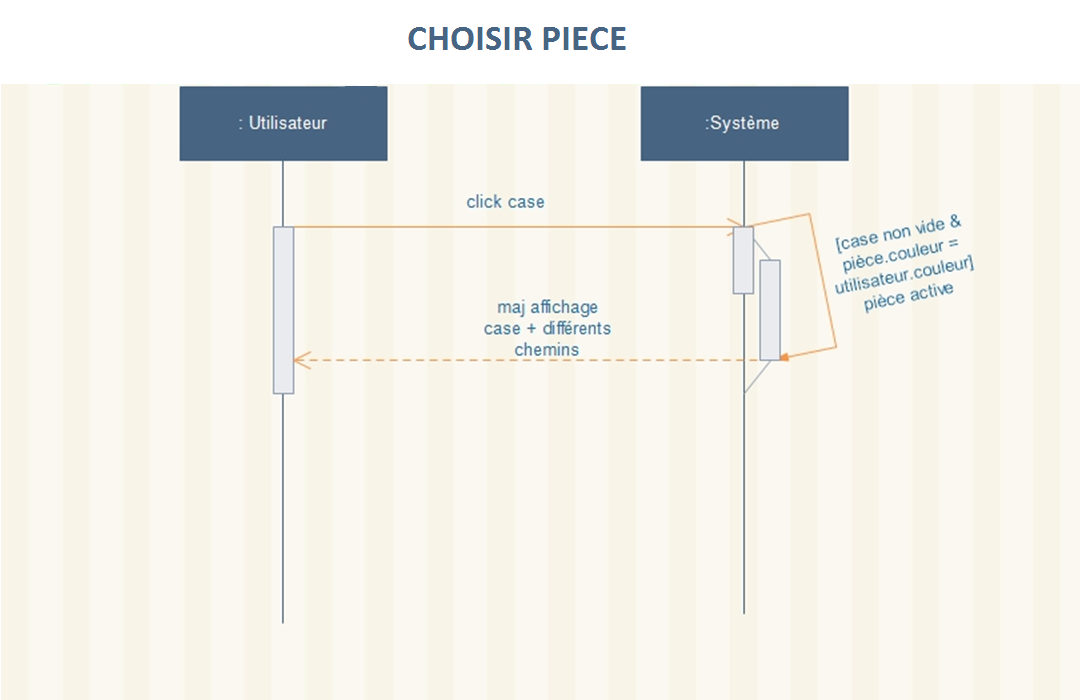
\includegraphics[width = 35em, height=20em]{images/seq/choisir_piece.png}
  %\caption{}
\end{center}
\end{figure*}

\begin{figure*}[ht]
\begin{center}
  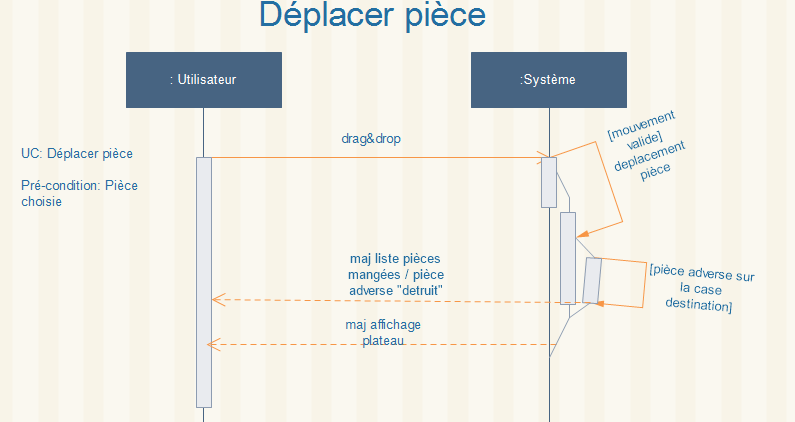
\includegraphics[width = 35em, height=20em]{images/seq/deplacer_piece.png}
  %\caption{}
\end{center}
\end{figure*}

\begin{figure*}[ht]
\begin{center}
  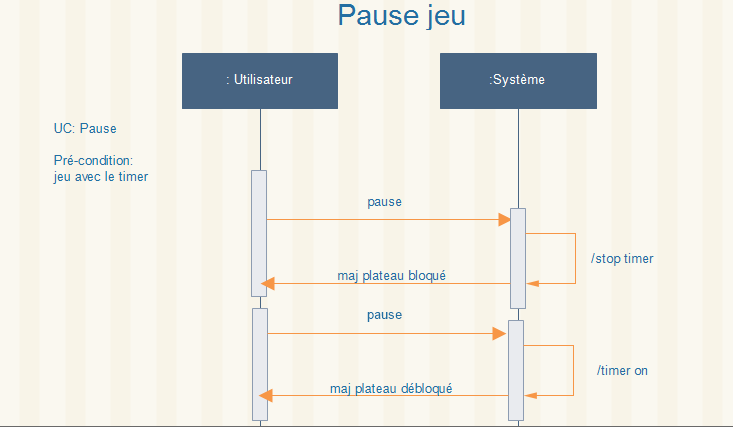
\includegraphics[width = 35em, height=20em]{images/seq/pause.png}
  %\caption{}
\end{center}
\end{figure*}

\begin{figure*}[ht]
\begin{center}
  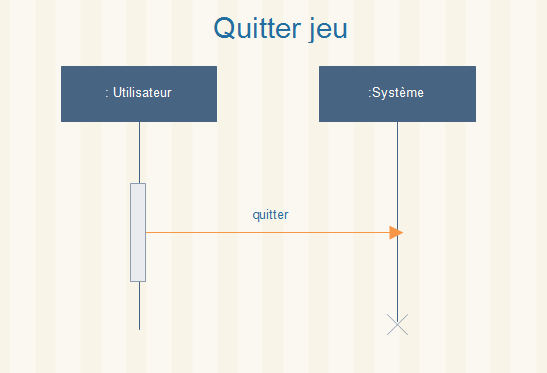
\includegraphics[width = 35em, height=20em]{images/seq/quitter.png}
  %\caption{}
\end{center}
\end{figure*}

\begin{figure*}[ht]
\begin{center}
  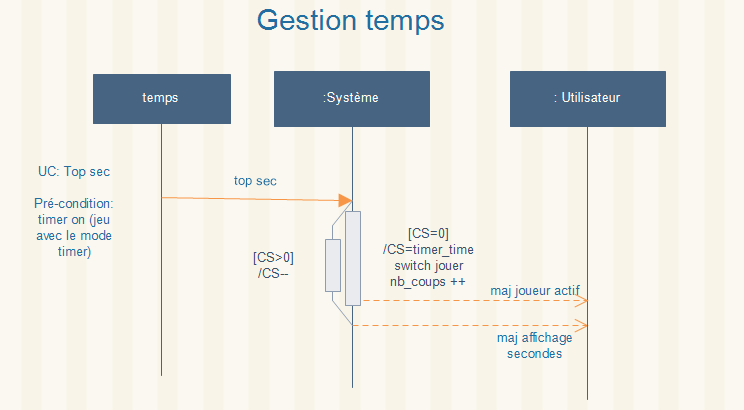
\includegraphics[width = 35em, height=20em]{images/seq/gestion_temps.png}
  %\caption{}
\end{center}
\end{figure*}

\begin{figure*}[ht]
\begin{center}
  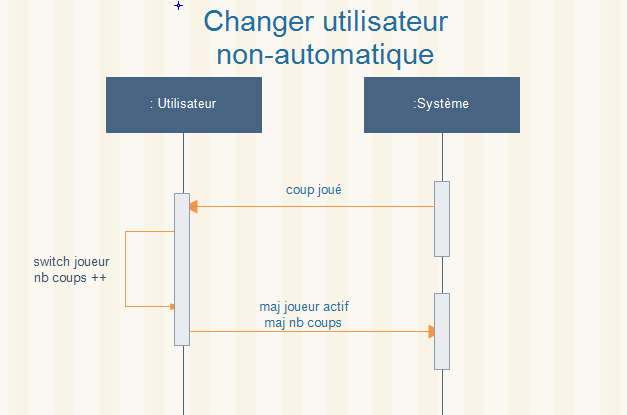
\includegraphics[width = 35em, height=20em]{images/seq/changer_joueur.png}
  %\caption{}
\end{center}
\end{figure*}


\newpage
\section*{Diagramme de classe}
\begin{figure*}[ht]
\begin{center}
  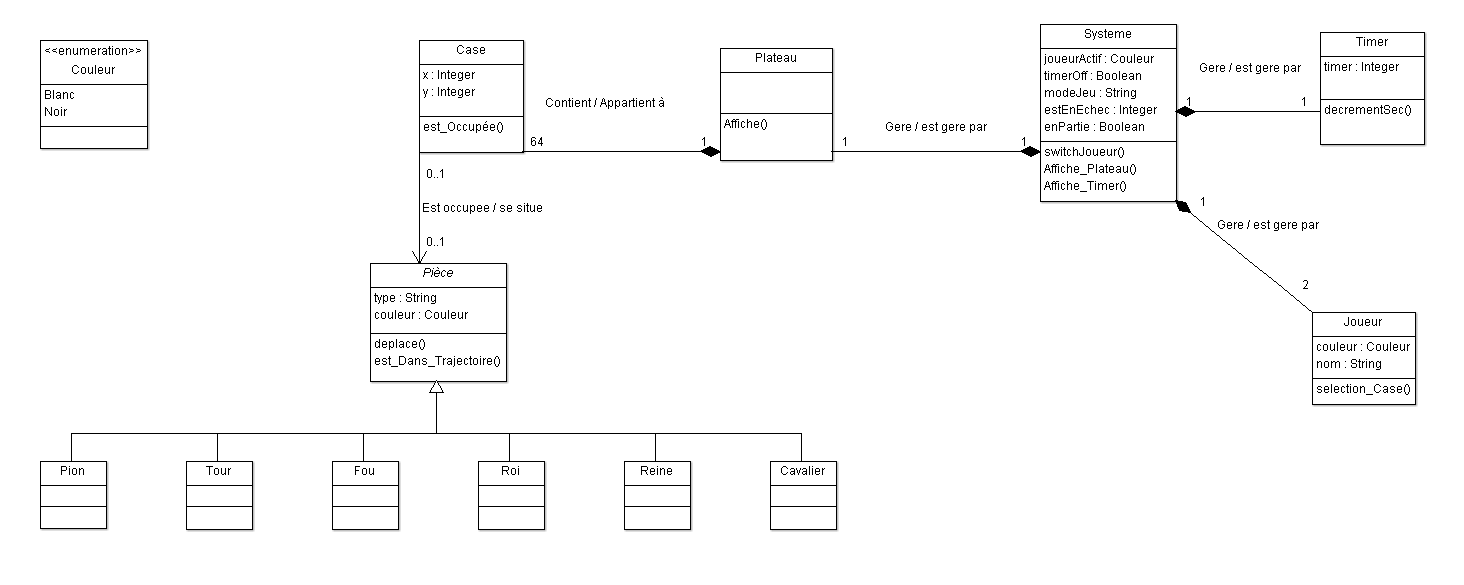
\includegraphics[width = 35em, height=60em]{images/classe/Diagrammedeclasses.png}
\end{center}
\end{figure*}
\maketitle
\chapter*{Architecture logique du logiciel}
\section*{Modèle-Vue-Contrôleur}
On a choisi ce modèle car :
\\-il y a beaucoup d'interactions avec l’utilisateur à travers l’IG susceptible de modifier la vue en interprétant les requêtes,
\\-certains mécanismes (règles du jeu) doivent interagir entre contrôleur et la vue, ce qui n’est pas possible avec une architecture en couche.

\maketitle
\chapter*{Description de l'incrément choisi}
{\tt IG} : en 2D; fenêtre des scores ; fenêtre des règles du jeu ; fenêtre de jeu
\\{\tt Mode de jeu} : 2 joueurs
\\{\tt Moteur de jeu} : sélection d'une case jouable ; prise d'une pièce adverse ; mouvements classiques ; échec/échec et mât 
\newpage
\section*{Diagramme d'états-transition}
\begin{figure*}[ht]
\begin{center}
  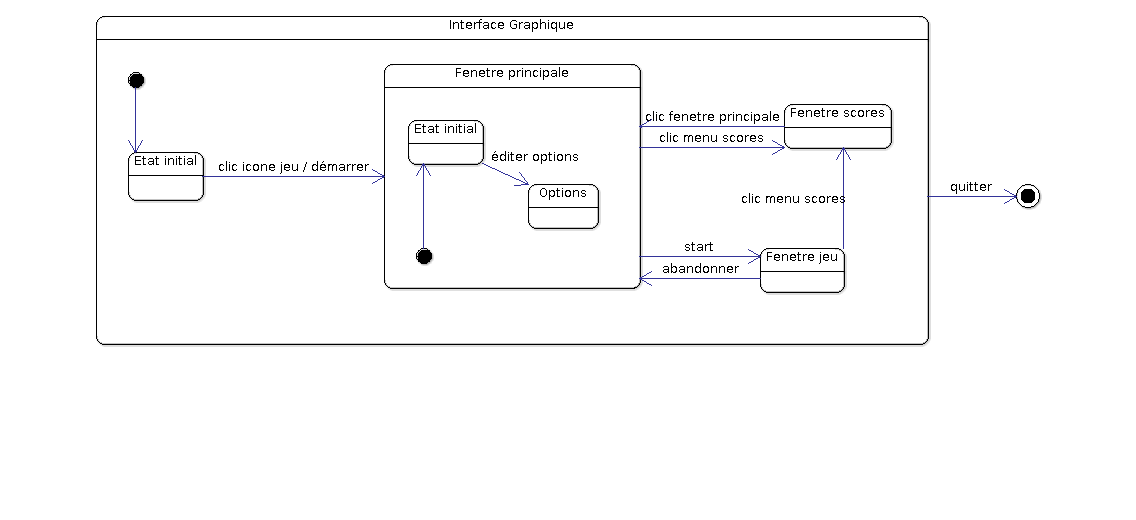
\includegraphics[width = 35em, height=25em]{images/plop/plop1.png}
\end{center}
\end{figure*}

\begin{figure*}[ht]
\begin{center}
  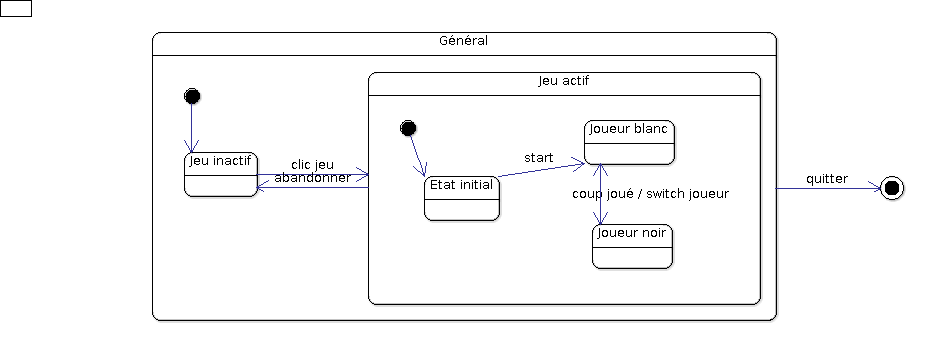
\includegraphics[width = 35em, height=25em]{images/plop/plop3.png}
\end{center}
\end{figure*}

\begin{figure*}[ht]
\begin{center}
  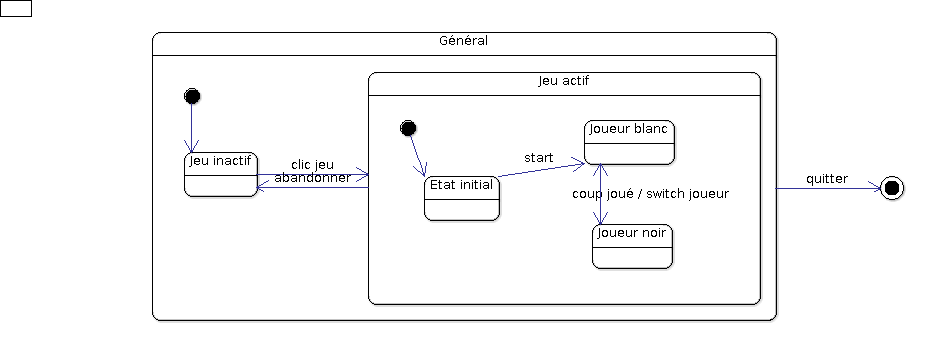
\includegraphics[width = 35em, height=25em]{images/plop/plop3.png}
\end{center}
\end{figure*}
\newpage
\section*{Diagramme de classe}
\clearpage
\begin{figure*}[ht]
\begin{center}
  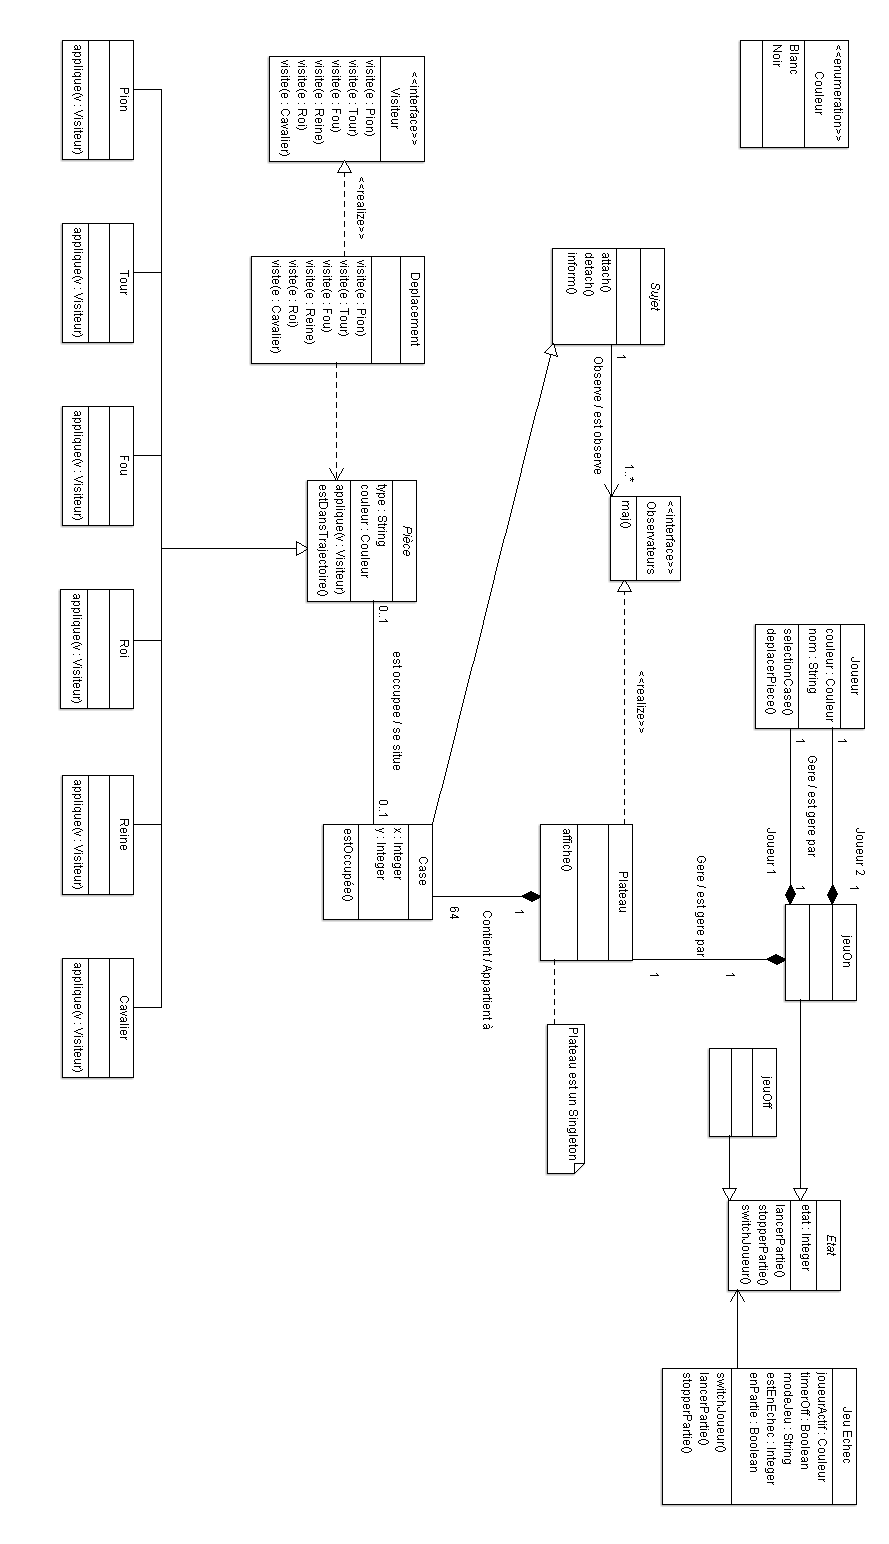
\includegraphics[width = 35em, height=60em]{images/classe/Diagrammedeclasseslogiciel.png}
\end{center}
\end{figure*}
\maketitle
\chapter*{Manuel de l'utilisateur pour l'incrément}

\section*{Débuter une partie}
L'utilisateur doit cliquer sur le menu déroulant {\it File} puis sur le sous menu {\it New Game} afin de commencer une nouvelle partie.
\section*{Terminer une partie}
L'utilisateur a plusieurs façons de terminer la partie :
\\la plus brutale est de fermer la fenêtre de jeu, 
\\ la plus naturelle est d'attendre la fin du jeu en gagnant ou en perdant la partie. 
\section*{Déplacer une pièce}
Sélectionner votre pièce en cliquant dessus avec la souris puis en maintenant le bouton enfoncé, déplacer celle-ci jusqu'à la case souhaitée (drag and drop).
\\Si cette case est valide, le mouvement est validé et votre pièce déplacée.
\\Une case est valide si elle respecte les possibilités de mouvement de la pièce sélectionnée.
\section*{Prendre une pièce adverse}
Déplacer votre pièce (cf section précédente), si son mouvement est correct et que sa case d'arrivée correspond à une case ou se situe une pièce adverse alors vous "prenez" la pièce adverse.
\\ Attention au cas particulier des pions qui prennent en diagonale, ie sur la case de la ligne supérieure et de la colonne droite ou gauche.
\section*{Voir les règles}
Cliquer sur le menu déroulant {\it File} puis sur le sous menu{\it Rules}.
\section*{Voir les scores}
Cliquer sur le menu {\it Scores}.

\maketitle
\chapter*{Bilan sur les outils de modélisation utilisés}

\section*{Problèmes rencontrés}
Nous avons utilisé ArgoUML pour construire les diagrammes de classes et les diagrammes d'états-transitions. Ce logiciel est facile à prendre en main mais le tracé des diagrammes de classes a été laborieux. En effet le déplacement des flèches est délicat à réaliser.
\\Pour les diagrammes de séquence nous avons utilisé \"?\", il était plus facile de tracer les diagrammes séquences qu'avec ArgoUML.


\section*{Solutions apportées}
ArgoUML : beaucoup de patience et de self-control.
\\:
\end{document}
